\documentclass[french]{beamer}

\usepackage[utf8]{inputenc}
\usepackage[T1]{fontenc}
\usepackage{lmodern}
\usepackage{amsmath, amssymb}
\usepackage[frenchb]{babel}

\setbeamertemplate{itemize item}[ball]
\setbeamertemplate{itemize subitem}[triangle]
\setbeamertemplate{itemize subsubitem}[circle]

% CHOIX DU THEME et/ou DE SA COULEUR
% => essayer différents thèmes 
% voir http://mcclinews.free.fr/latex/beamergalerie/completsgalerie.html
\usetheme{PaloAlto}
% \usetheme{Madrid}
% \usetheme{AnnArbor}
% \usetheme{Copenhagen}

% voir http://mcclinews.free.fr/latex/beamergalerie/colorgalerie.html
% \usecolortheme{crane}
% \usecolortheme{seahorse}
% \usecolortheme{albatross}
\usecolortheme{dolphin}
% \useoutertheme[left]{sidebar}


% Pour le TITLEPAGE
\title{\textsc{MuSIK}}
\subtitle{Musical Software Instruments for Kids}
\date{Avril 2014}
\institute{\textsc{ENSEIRB-MatMeca}}
\logo{
\includegraphics[height=10mm]{logo.png}}

\begin{document}

\begin{frame}
  \titlepage
\end{frame}

\begin{frame}{\textsc{\Large Projet au Fil de l'Année 2014}\\[0.5cm]}
  \begin{center}
    Clé USB de logiciels pour élèves d'école de musique\\
    \begin{minipage}{0.5\textwidth}
      \visible<2->{
        \begin{flushleft} \large
          \emph{Auteurs:}\\
          \textsc{Dando} Louis-Marie\\
          \textsc{Fatsawo} Yoan\\
          \textsc{Jomard} Arnaud\\
          \textsc{Migot} Jean-Luc\\
          \textsc{Milhet} Louis\\
          \textsc{Monmarche} Louis\\
        \end{flushleft}
      }
    \end{minipage}
    \begin{minipage}{0.4\textwidth}
      \begin{flushleft} \large
        \visible<3->{
          \emph{Responsable Pédagogique :} \\
          \textsc{Gloess} Paul-Yves\\[0.5cm]
        }
        \visible<4->{
          \emph{Clients :}\\
          \textsc{Thibault} Samuel
          \textsc{Furher} Emmanuel
          \textsc{Durand} Michel
        }
      \end{flushleft}
    \end{minipage}
    \\[2cm]
    \large Mars 2014
  \end{center}
\end{frame}

\begin{frame}{Sommaire}
  \tableofcontents
\end{frame}

\section{Présentation}
\begin{frame}
\tableofcontents[currentsection]
\end{frame}
\begin{frame}
c'est la présentation
\end{frame}

\section{Notre solution : la clé USB}
\begin{frame}
\tableofcontents[currentsection]
\end{frame}

\begin{frame}
  \frametitle{Les Outils}
  \begin{columns}[t]
    \begin{column}{10cm}
      \begin{exampleblock}{Les outils proposés}
	\begin{itemize}
	\item VLC Media Player : un lecteur de média.
	\item Audacity : un éditeur audio.
	\item Metronomix : un métronome.
        \item MuseScore : un éditeur de partition.
	\end{itemize}
      \end{exampleblock} 
    \end{column}
  \end{columns}
  \begin{figure}[!h]
    \centering{
      
\includegraphics[width = 0.15\textwidth]{../images/tool_vlc.png}
      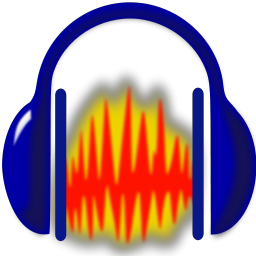
\includegraphics[width = 0.15\textwidth]{../images/tool_audacity.png}
      
\includegraphics[width = 0.15\textwidth]{../images/tool_metronomix.png}
      
\includegraphics[width = 0.15\textwidth]{../images/tool_score.png}
    }
    \label{VLC, Audacity, Metronomix et MuseScore} 
    \caption{VLC, Audacity, Metronomix et MuseScore}
  \end{figure}        
\end{frame}

\begin{frame}
  \frametitle{Le Quizz}
  Le Quizz est composé de 2 écrans :
  \begin{columns}[t]
    \begin{column}{10cm}
      \begin{exampleblock}{L'écran de selection}
	\begin{itemize}
        \item Choix du thème.
        \item Choix de la difficulté.
        \end{itemize}
      \end{exampleblock} 
    \end{column}
  \end{columns}  

  \begin{columns}[t]
    \begin{column}{10cm}
      \begin{exampleblock}{L'écran de quizz}
	\begin{itemize}
        \item Question au format texte, image ou son.
        \item Réponse à choix multiples.
        \item Explication du professeur.
        \item Temps limité.
        \end{itemize}
      \end{exampleblock} 
    \end{column}
  \end{columns}  
\end{frame}

\begin{frame}
  \frametitle{Le Jeu}
  Le jeu s'inspire du classique \textbf{Space Invaders}.
  \begin{itemize}
    \item Le joueur contrôle un vaisseau qui doit attaquer des notes de musique.    \item La note à attaquer change régulièrement.
    \item La difficulté augmente en fonction du cursus musical des élèves.  
  \end{itemize}

  \begin{figure}[!h]
    \centering
    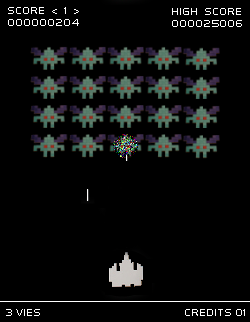
\includegraphics[height = 0.5\textheight]{img/Space_Invaders.png}
    \label{Space Invaders} 
    \caption{Space Invaders}
  \end{figure}
\end{frame}

\begin{frame}
  \frametitle{Administration et aide}
 \begin{columns}[t]
    \begin{column}{10cm}
      \begin{exampleblock}{Les différents menus}
	\begin{itemize}
        \item Un menu qui permet de modifier les données du quizz ou du jeu.
        \item Choix de la langue.
        \item Aide pour l'utilisateur.
        \end{itemize}
      \end{exampleblock} 
    \end{column}
  \end{columns}  
\end{frame}


\section{Organisation}

\begin{frame}
\tableofcontents[currentsection]
\end{frame}
\begin{frame}
lorem lipsum
\end{frame}

\section{Conception et développement}

\begin{frame}
\tableofcontents[currentsection]
\end{frame}
\begin{frame}
lorem lipsum
\end{frame}

\section{Problèmes rencontrés}

\begin{frame}
\tableofcontents[currentsection]
\end{frame}
\begin{frame}
lorem lipsum
\end{frame}

\section{Perspectives d'évolution}

\begin{frame}
\tableofcontents[currentsection]
\end{frame}
\begin{frame}
lorem lipsum
\end{frame}

\section{Conclusion}

\begin{frame}
\tableofcontents[currentsection]
\end{frame}
\begin{frame}
tadamm
\end{frame}

\end{document}